\section{System's Perspective}

\subsection{Design}
To develop our version of MiniTwit, we have chosen to use the programming language Go. We are using a toolkit called Gorilla that includes a number of different packages, that each help with different things regarding web development. We use the library called GORM to interact with our PostgreSQL database instead of writing our own SQL queries. We use Prometheus to monitor our application - and Grafana to give us a dashboard with the Prometheus data. To log things like error messages, we use the ELK stack.


\subsection{Architecture}

\subsubsection{Components and connectors}
Our system is containerized using docker and deployed with DigitalOcean, which enables the user to access and use the application.
Our API and app are connected to the database container. We use Caddy as our reverse proxy. Caddy receives traffic and redirects it to either the API, app, Grafana, or Kibana, using the same ports for all four services.

\begin{figure}[H]
    \centering
    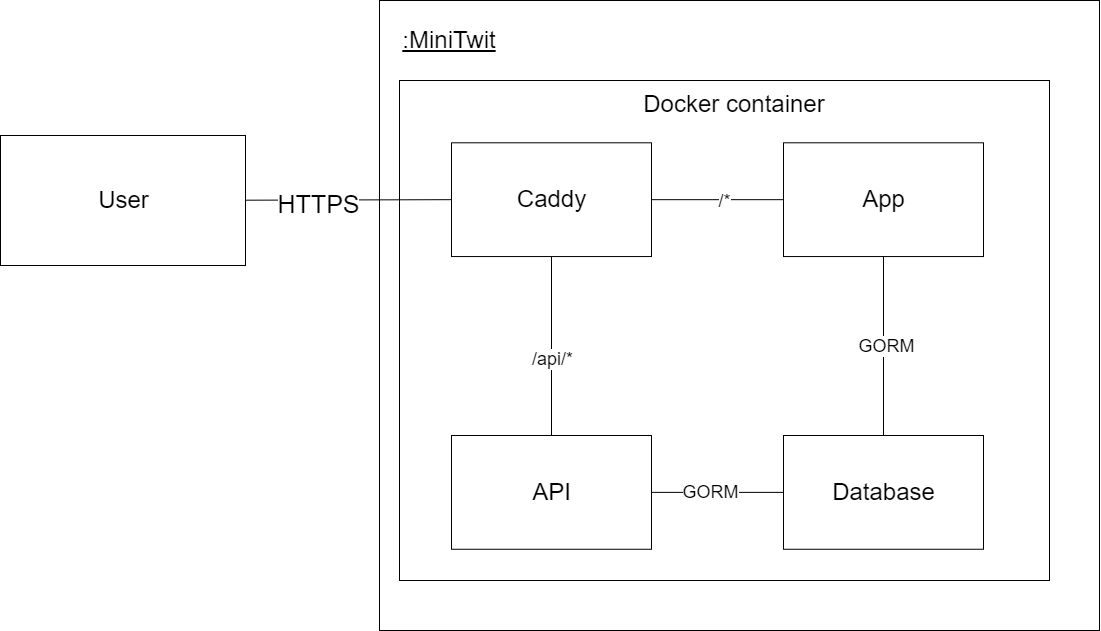
\includegraphics[scale=0.40]{images/C&C_diagram.png}
    \caption{Diagram showing an overview of our components and connectors.}
    \label{fig:CCDiagram}
\end{figure}

\subsubsection{Module Viewpoints}
\subsubsection*{Packages}

The system consists of three packages: \textit{src}, \textit{CircleCI} and \textit{Docker}. The packages and their dependencies are visualized in figure \ref{fig:packages}.

The \textit{src} package contains the system logic relevant to user actions in the app and API. The app handles user inputs from the MiniTwit website, whereas the API handles HTTP requests through exposed endpoints. \textit{src} also contains the monitoring and the controller packages.

The \textit{monitoring} package contains two things. First and foremost, the monitoring infrastructure is set up with the Prometheus package.
The Prometheus Promauto functionality is used to define what metrics to track. We chose it because it sets up an easily extendable code structure.
Secondly, the function MiddlewareMetrics starts a timer and measures CPU usage before serving the http request it is handling. After having served the HTTP request it increments the request count and records the duration of the HTTP request. 

The \textit{controller} simply defines the structs for the database, to connect to the database, query a users ID from a username and hash passwords.
\newline
For a full overview of the entire \textit{src} package, see appendix \ref{appendix:CCDiagram}

The \textit{Docker} package is not tied to MiniTwit functionality. Its purpose is to contain the instructions for initialization of our different Docker containers when we deploy the system. This means that it contains a variety of file types. Naturally, it contains the .Dockerfile for the app and API. Furthermore, it contains .yml files with launch settings for our monitoring tools. The \textit{/grafana} directory also includes .json files that define the UI for its dashboard. \newline
These files are run at every system initialization, building the containers, based on the data carried in the package.

Finally, the \textit{CircleCI} package contains the functionality for CI/CD. It is linked to our GitHub repository, meaning that every time we merge a pull request into the MiniTwit repository's main branch, the setup in the \textit{Docker} package is run.

\begin{figure}[H]
    \centering
    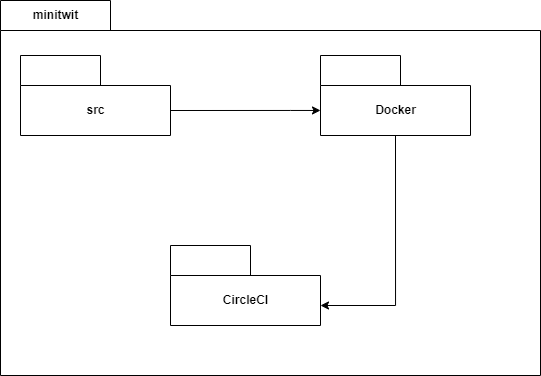
\includegraphics[scale=0.60]{images/packages.png}
    \caption{This diagram shows the outermost layer of the Minitwit packages and their dependencies.}
    \label{fig:packages}
\end{figure}


\subsubsection*{Src}
The overview of our \textit{src} package is seen in figure \ref{fig:src} which visualizes the dependencies of our \textit{API} and \textit{App}.

\begin{figure}[H]
    \centering
    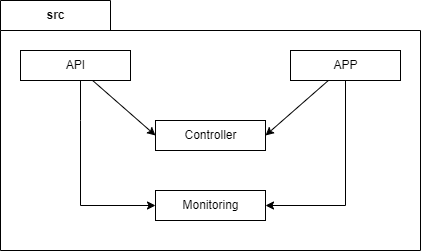
\includegraphics[scale=0.75]{images/src.png}
    \caption{The diagram shows the dependencies between the API and app in the \textit{src} package.}
    \label{fig:src}
\end{figure}

\newpage

\subsubsection*{Class overview of App}

Our App consists of the following:

\begin{itemize}
    \item Main.go $\rightarrow$ our back-end functionality of the application
    \item Front-end, consisting of 4 HTML files
    \begin{itemize}
        \item Layout.html
        \item login.html
        \item register.html
        \item timeline.html
    \end{itemize}
    \item a single CSS file responsible for the UI-design of our front-end
\end{itemize}

Our app exposes HTTP-endpoints for the following use cases:

\begin{itemize}
    \item \texttt{/} $\rightarrow$ If user logged in, loading personal timeline, if not logged in, redirecting to \texttt{/public}
    \vspace{0.5em}
    \item \texttt{/favicon.ico} $\rightarrow$ prevents the app from thinking favicon.ico is a user
    \vspace{0.5em}
    \item \texttt{/public} $\rightarrow$ loads the public timeline
    \vspace{0.5em}
    \item \texttt{/add\_message} $\rightarrow$ posting message on the web service
    \vspace{0.5em}
    \item \texttt{/login} $\rightarrow$ login opportunity for users
    \vspace{0.5em}
    \item \texttt{/register} $\rightarrow$ registration opportunity for users
    \vspace{0.5em}
    \item \texttt{/logout} $\rightarrow$ opportunity to log out of the web service
    \vspace{0.5em}
    \item \texttt{/\{username\}} $\rightarrow$ load the timeline of the given user
    \vspace{0.5em}
    \item \texttt{/\{username\}/follow} $\rightarrow$ logged in user wanting to follow user called  \texttt{\{username\}}
    \vspace{0.5em}
    \item \texttt{/\{username\}/unfollow} $\rightarrow$ logged in user wanting to unfollow user called\\ \texttt{\{username\}}
\end{itemize}

In order to display data in the front-end, we make use of the struct \texttt{TimelineData}, which acts as a container for the data fetched from the database. The struct \texttt{SessionData} is used to keep track of the data associated with the current session in the application. In other words, this is the struct whose field, \texttt{Flashes}, is injected into the frontend, such that nothing is directly exposed to the front-end. This hides the back-end functionality, improving security of the site as well as keeping the code less coupled, such that changes in one part do not break others. To load the data on the frontend, we use the Go package \textit{Go/Template} which allows for Go code to be loaded directly in the HTML without the need for any JavaScript.

\newpage

\subsubsection*{Class overview of API}
The API makes use of HTTP requests by exposing HTTP-endpoints in order for the internal logic to handle the HTTP requests. Every endpoint has been kept according to the initial Python application.  
Our API has exposed endpoints for the following HTTP requests:
\begin{itemize}
    \item Registering users (POST) /api/register - if success, returns HTTP response code 204. If failing, returns HTTP response 400.
    \item Following a user (POST / GET) /api/follws/\{username\} - the method is checking if already followed (GET) and following / unfollowing (POST)  - if success, returns HTTP response code 204. If failing, returns HTTP response 404.
    \item Latest message (GET) /api/latest  - returns the ID of the latest message from the application.
    \item Messages per user (GET) /api/msgs/\{username\} - if success, returns HTTP response code 204. If failing, returns HTTP response 405.
    \item Messages (feed) (GET) /api/msgs - if success, returns HTTP response code 204. If failing, returns HTTP response 405.
\end{itemize}

The API is meant to be run within a simulator environment, which acts as if the API is being accessed by real users. In our case, the API has failed quite a lot (around 90-95\%), which is due to downtime of our database (4 days). We are suspecting that a lot of the users were registered during these days and therefore we had a lot of errors. The errors arising from \textit{user does not exist} has also caused the problem that it camouflaged any downstream errors. Due to the fact that it does not follow good DevOps principles to just register users (by using the "username" property in some endpoints and therefore allowing null-values in the database, which is not a maintainable solution) when they did not exist, we were unable to find a way of resolving this in a proper manner.

\newpage

\subsubsection{Deployment}
The deployment diagram below (see figure \ref{fig:deployment_diagram}) visualizes the dependencies between software containers, stored in Docker containers, and the physical hardware that runs it. The system is run on a virtual machine hosted by DigitalOcean. The virtual machine runs Ubuntu 20.04 LTS and the OS runs the system in a Docker daemon that contains individual Docker containers and Docker networks. 
\newline
The two Docker networks are separated into logical units. The first unit is the main-network, which contains the system logic, monitoring tools, and the database. The second network container, elk-network, contains the tools used to create logs. As the ELK setup does not need to communicate with any of the applications, it does not need to be in the same network. It works by Filebeat reading directly from the system directory that contains the logs from Docker containers, which is mounted as a Docker volume.

\begin{figure}[H]
    \centering
    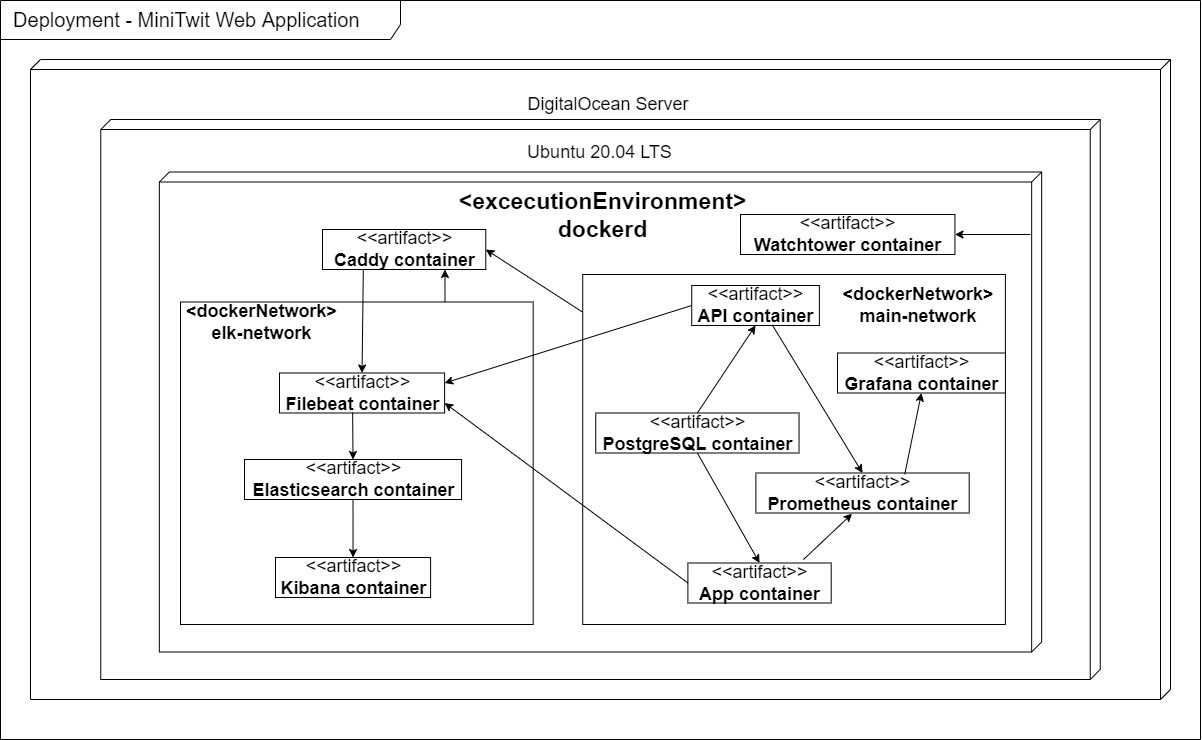
\includegraphics[scale=0.37]{images/deployment_diagram.png}
    \caption{The deployment diagram highlights how the software elements are mapped to the hardware that it is hosted on.}
    \label{fig:deployment_diagram}
\end{figure}

\newpage

\subsection{Dependencies}
\begin{itemize}
    \item Go 1.18.x
    \vspace{0.5em}
    \item DigitalOcean: Our hosting service.
    \vspace{0.5em}
    \item Docker: Service for containerizing software.
    \vspace{0.5em}
    \item Docker Compose: Tool that gives instructions to Docker on what images to initialize when deploying the system. 
    \vspace{0.5em}
    \item CircleCI: A platform for continuous integration and deployment.
    \vspace{0.5em}
    \item PostgreSQL: The relational database system \vspace{0.5em}
    \item Gorilla/mux: A http request router and dispatcher which we use for matching incoming request to their respective handlers. 
    \vspace{0.5em}
    \item GORM: Go library used for creation of relational database schema and migration, as well as providing CRUD operations. 
    \vspace{0.5em}
    \item Prometheus: Our monitoring software.
    \vspace{0.5em}
    \item Grafana: An analytics and visualization tool which is hooked up to Prometheus.
    \vspace{0.5em}
    \item ELK: A Docker Image providing the following services: 
    \vspace{0.5em}
    \begin{itemize}
        \item Elasticsearch: used for its index log data.
        \vspace{0.5em}
        \item Filebeat: Collects logging data and forwards it to Elasticsearch.
        \vspace{0.5em}
        \item Kibana: Visualization and navigation tool for the data stored in Elasticsearch. 
        \vspace{0.5em}
    \end{itemize}
    \item Caddy: Proxy and web server service. We use it for reverse proxying.
    \vspace{0.5em}
    \item Watchtower: A service for checking updates for Docker images and updating Docker containers.
\end{itemize}

\subsection{Important interactions of subsystems}
We use Docker Compose to run multiple Docker containers for our system, such as MiniTwit, ELK, Prometheus, etc. For automating the process of updating images, we use Watchtower. 


For logging we have set up our Docker Compose file to create containers for the three ELK images; Elasticsearch, Filebeat, and Kibana. Filebeat is the container that observes and ships data to Elasticsearch. Kibana then receives the data from Elasticsearch and visualizes it.  


When new features are pushed to the GitHub repository's main branch, CircleCI triggers and re-deploys the system. 


We monitor our application with Prometheus, which collects metrics by scraping from a selection of HTTP endpoints. These metrics are then stored on the Prometheus server, and can be exported or visualized with Grafana.

\subsection{Current state of our system}
%Describe the current state of your systems, for example using results of static analysis and quality assessment systems
SecureGo notified that the .md5 hashing algorithm is weak. Our system still uses it, as it is a requirement for Gravatar URLs.

At the end of development, we have judged our system according to our chosen metrics, described in section \ref{CI/CD}.
\begin{itemize}
    \item Maintainability - The code base has been left in a maintainable state. It is easy to navigate and understand. The packages divide the system in logical units.
    \item Testability  - We did not manage to implement unit testing in time. However, we do static analysis on all branches and also build and deploy for each pull request to main.
    \item Portability - The portability of the system is difficult to estimate without unit or integration testing. Again, the static analysis and clean conventions combat this somewhat, though we are not completely satisfied yet.
    \item Reusability - We have managed to make our code reusable and avoiding redundant code. An example is our controller, which has methods used by both our API and app.
    \item Technical debt - During the course of developing and maintaining Minitwit, we tried to minimize our accrued technical debt. The most mention-worthy debt, is that our Docker swarm is stopping our monitoring and logging from working. As such, the production branch, at the date of delivery, is not using swarm, to prioritize monitoring.  
\end{itemize}

\subsection{License compatibility}
Our MiniTwit application is licensed under the AGPLv3 license. After running the tool \textit{\href{https://github.com/uw-labs/lichen}{lichen}} on our code, we found no license violations. AGPLv3 is the most copy-left license that we know of, meaning that almost all other FOSS licenses are compatible with it.